\section{Problem Statement}\label{sec:problem-statement}
\begin{figure*}[!t]
  \centering
  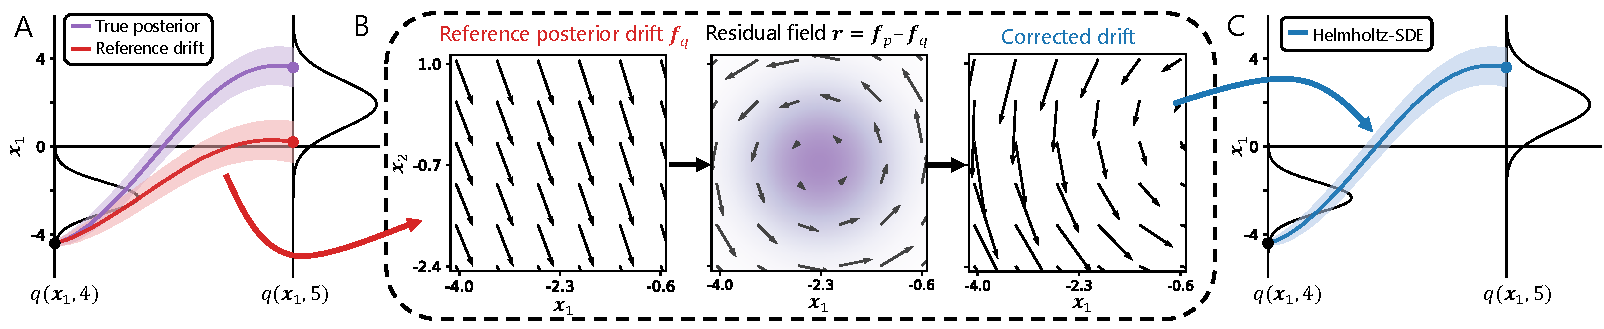
\includegraphics[width=\textwidth]{figs/fig1-overview.pdf}

  \caption{
  Overview of Helmholtz-SDE.
  \textbf{A}:
    Existing simulation-free VI algorithms commit to a single drift (red) for each set of one-time marginals (black). This choice induces transition distributions that can differ from those of the true posterior (purple), even when the one-time marginals agree.
    \textbf{B}:
    Helmholtz-SDE takes a drift consistent with a set of one-time marginals, then corrects it by a vector field that preserves the marginals.
    \textbf{C}: The resulting approximation (blue) better matches the posterior.
    }
  \label{fig:spiral-overview}
  \vspace{-1em}
\end{figure*}

\paragraph{Model.}
We study \emph{latent stochastic differential equation} (SDE) models, in which a $K$-dimensional latent state $\mbx(t)$ evolves over the interval $0 \leq t \leq T$ and gives rise to $D$-dimensional observations $\mby(t_n)$ at times $\{t_n\}_{n=1}^N$. 
Let $\mbtheta$ denote the full collection of model parameters, including the parameters of the prior and the likelihood.
The prior over the latent state is the solution to an SDE
\begin{equation}\label{eqn:prior_sde} 
\bbP_{\mbtheta}\!\!:\; d\mbx(t) = \mbf_p(\mbx(t)| \mbtheta) dt + \mbSigma(\mbtheta)^{1/2} d\mbw(t), \quad  \mbx(0) \sim p(\mbx, 0 | \mbtheta), \quad 0 \leq t \leq T,
\end{equation}
where $\mbf_p(\cdot | \mbtheta)\!: \bbR^K \to \bbR^K$ is the drift function, 
$\mbSigma(\mbtheta)^{1/2}$ is the diffusion coefficient,
$(\mbw(t))_{0 \leq t \leq T}$ is a standard $K$-dimensional Brownian motion, 
and $p(\mbx, 0 | \mbtheta)$ is the initial state distribution. 
We denote the marginal density of $\bbP_{\mbtheta}$ at time $t$ by $p(\mbx, t | \mbtheta)$.
For simplicity of presentation, we restrict notation to a time-independent drift and a state- and time-independent diffusion coefficient.

We observe data $\cD = \{(t_n, \mby(t_n))\}_{n=1}^N$ representing noisy readouts of the latent state. 
These observations are conditionally independent given the latent state:  $p(\mby | (\mbx(t))_{0 \leq t \leq T}, \mbtheta) = \prod_{n=1}^N p(\mby(t_n) | \mbx(t_n), \mbtheta)$, where $\mby = \{\mby(t_n)\}_{n=1}^N$.
We describe our technical assumptions on the generative model in \Cref{app:subsec:assumptions}.

There are two goals in latent SDE models: (i) to learn the parameters $\mbtheta$ that maximize $\log p(\mby | \mbtheta)$; and (ii) to infer an approximate posterior over the latent trajectory $(\mbx(t))_{0 \leq t \leq T}$ given the data $\cD$ and parameters $\mbtheta$.
In practice, one may have multiple trials $\{\mby^{(m)}\}_{m=1}^{M}$, each representing an independent sample from the probabilistic model. 
In this case, the model parameters $\mbtheta$ are learned using all trials, and the posterior factorizes over trials. For simplicity, we suppress the trial index $m$.

\paragraph{Intractability.}
Both goals of learning and inference are generally intractable. 
For learning, evaluating the marginal likelihood $p(\mby | \mbtheta)$
involves marginalizing over the prior on latent trajectories \eqref{eqn:prior_sde}; this integral cannot be evaluated in closed form.
For inference, the posterior law is the solution to an SDE with the same diffusion coefficient $\mbSigma^{1/2}$ as the prior and drift obtained by solving a linear partial differential equation \cite{kushner1964differential, stratonovich1965conditional, pardoux1982equations,archambeau2011approximate}. 
In nonlinear or non-Gaussian settings, the posterior drift is unavailable in closed form, and solving the associated PDE can be computationally prohibitive even for small $K$.

\section{Background}\label{sec:background}
Variational inference (VI) provides a tractable framework for joint learning and inference in latent SDEs. We first describe the variational objective and survey existing VI algorithms. We then identify a class of stochastic VI algorithms that avoid sequential simulation, the setting of our method.

\subsection{Variational inference for latent SDE models}\label{subsec:variational_inference}
Variational inference (VI) approximates the intractable posterior with a distribution belonging to a tractable family, known as a  \emph{variational family} \cite{jordan1999introduction, blei2017variational}. 
For latent SDEs, we consider the family $\cQ$ comprised of diffusion processes
\begin{equation}\label{eqn:variational_family}
    \bbQ_{\mbphi}\!\!:\; d \mbx(t) = \mbf_q(\mbx(t), t | \mbphi) dt + \mbSigma(\mbtheta)^{1/2} d\mbw(t), \quad \mbx(0) \sim q(\mbx, 0 | \mbphi), \quad 0 \leq t \leq T,
\end{equation}
where the variational parameters $\mbphi$ specify the posterior drift $\mbf_q(\mbx, t| \mbphi)$ and the initial state distribution $q(\mbx, 0 | \mbphi)$.
This family is chosen because, when $\mbf_q(\mbx, t | \mbphi)$ and $q(\mbx, 0 | \mbphi)$ are sufficiently expressive,
the exact posterior will belong to $\cQ$ \citep[see, e.g.,][]{hu2025sing}.

We minimize the negative evidence lower bound (ELBO) over distributions in $\cQ$,
\begin{equation}\label{eqn:elbo}
\begin{aligned}
   \cL(\mbtheta,\mbphi) &= \underbrace{\sum_{n=1}^N {-}\bbE_{\bbQ_{\mbphi}} \log p(\mby(t_n) | \mbx(t_n), \mbtheta)}_{\cL_{\mathrm{rec}}} 
   + \underbrace{\KL{q(\mbx, 0 | \mbphi)}{p(\mbx, 0 | \mbtheta)}}_{\cL_{\mathrm{init}}}  + \\
   &\underbrace{\frac{1}{2}\int_0^{T} \bbE_{\bbQ_{\mbphi}} \|\mbSigma(\mbtheta)^{-1/2}\{\mbf_q(\mbx(t), t | \mbphi) - \mbf_p(\mbx(t)| \mbtheta)\}\|_2^2 dt}_{\cL_{\mathrm{path}}},
\end{aligned}
\end{equation}
where $\cL_{\mathrm{rec}}$ is the reconstruction loss, $\cL_{\mathrm{init}}$ is the KL divergence to the prior initial distribution, and $\cL_{\mathrm{path}}$ is the path-space KL divergence to the prior.

The negative ELBO is an upper bound on the negative marginal log likelihood $-\log p(\mby | \mbtheta)$, and the gap between them is the KL divergence between $\bbQ_{\mbphi}$ and the exact posterior.
Therefore, when the exact posterior is contained in $\cQ$ it is the unique minimizer of \cref{eqn:elbo}.
\Cref{app:subsec:elbo} gives a derivation.
However, unlike the negative log likelihood, the ELBO provides a tractable objective for learning  model parameters, which we seek to estimate by jointly optimizing with respect to $\mbphi$ and $\mbtheta$.

Existing VI algorithms for latent SDEs fall into two broad classes based on how they evaluate the negative ELBO \cref{eqn:elbo}: simulation-based and simulation-free.
We describe each in turn.

\subsection{Simulation-based VI}\label{subsec:sim-based}
\emph{Simulation-based} algorithms evaluate the path KL $\cL_{\mathrm{path}}$ over a discretization of the interval $[0, T]$ at each gradient step. 
When $\bbQ_{\mbphi}$ is restricted to a tractable family, such as a Gaussian process with affine $\mbf_q$ and state-independent $\mbSigma$, the marginals of $\bbQ_{\mbphi}$ can be computed by integrating an ODE \cite{archambeau2007gaussian, hu2025sing,archambeau2007variational, duncker2019learning, verma2024variational, kohs2021variational, wildner2021moment,park2024amortized, parkstochastic2026}.
When $\mbf_q$ is parameterized more flexibly, e.g., by a neural network \cite{li2020scalable, ryder2018black, tzen2019neural, kidger2021efficient, oh2024stable}, samples $\mbx(t) \sim \bbQ_{\mbphi}$ are obtained by simulating the variational SDE \eqref{eqn:variational_family}. 
In both cases, the time complexity per gradient step scales with the discretization of $[0, T]$, introducing a tradeoff between approximation fidelity and computational cost.

\subsection{Simulation-free VI}\label{subsec:sim-free}
\emph{Simulation-free} VI algorithms introduce two ideas to avoid discretizing the variational SDE and accelerate optimization of $\cL(\mbtheta, \mbphi).$
The first is to optimize
a Monte Carlo estimate of \cref{eqn:elbo}
\begin{equation*}
    \widehat{\cL}(\mbtheta, \mbphi) = -N \log p(\mby(t_n) | \mbx(t_n)) + \log\frac{q(\mbx(0), 0 | \mbphi)}{p(\mbx(0), 0 | \mbtheta)} + \frac{T}{2} \|\mbSigma(\mbtheta)^{-1/2}(\mbf_q(\mbx(t), t | \mbphi) - \mbf_p(\mbx(t) | \mbtheta))\|_2^2.
\end{equation*}
Here, $n \sim \cU(\{1, \dots, N\})$ is a random observation index, $t \sim \cU([0, T])$ is a random time, and $\mbx(0), \mbx(t_n), \mbx(t) \sim \bbQ_{\mbphi}$ are posterior samples.
The estimate $\widehat{\cL}(\mbtheta, \mbphi)$ avoids the sum over all observations in $\cL_{\mathrm{rec}}$, the integral over the full trajectory in $\cL_{\mathrm{path}}$, and the expectations over $\bbQ_{\mbphi}$ in all three terms of $\cL(\mbtheta, \mbphi)$. 
Compared to optimizing the negative ELBO, this approach introduces variance that is managed by averaging across Monte Carlo samples.
Because the estimate samples random times rather than full paths, optimization amounts to a stochastic VI algorithm \cite{hoffman2013stochastic}.

The second idea is to parameterize the drift $\mbf_q$ that defines $\bbQ_{\mbphi}$ implicitly through its one-time marginal distributions.
In order for optimizing $\widehat{\cL}(\mbtheta, \mbphi)$ to provide runtime benefits over optimizing the negative ELBO, we must be able to draw samples $\mbx(t) \sim \bbQ_{\mbphi}$ without simulating the variational SDE \cref{eqn:variational_family}.
This is achieved by reversing the usual construction of $\bbQ_{\mbphi}$: we first prescribe the marginal distribution of the posterior at any single time $\{q(\mbx,t|\mbphi)\}_{0 \leq t \leq T}$ and then choose a drift $\mbf_q$ compatible with those marginals.
One can sample $\mbx(t)$ from the posterior with time complexity that does not depend on $t$.

For example, SDE Matching (\citet{bartosh2025sde}) parameterizes the posterior as having Gaussian marginals, $q(\mbx,t|\mbphi)=\cN(\mbm(t|\mbphi),\mbS(t|\mbphi))$ and shows that a time-dependent, affine drift $\mbf_q(\mbx, t | \mbphi) = \mbA_q(t | \mbphi) \mbx + \mbb_q(t | \mbphi)$ defines a variational SDE with precisely these marginals.\footnote{The framework proposed by \citet{bartosh2025sde} can in principle support non-Gaussian one-time marginals, but the method is instantiated and evaluated only with Gaussian marginals. See \Cref{app:subsec:svise-sde-compare} for further discussion.}
A compatible drift is readily computed from $\mbm(t|\mbphi)$ and $\mbS(t|\mbphi)$ as
{\small
\begin{equation}\label{eqn:sym-sqrt-reference}
    \mbf_q(\mbx,t|\mbphi) = \left[\left(\frac{d}{dt}\mbS(t|\mbphi)^{1/2} \right) \mbS(t|\mbphi)^{-1/2} - \frac{1}{2}\mbSigma(\mbtheta)\mbS(t|\mbphi)^{-1} \right][\mbx(t)-\mbm(t|\mbphi)] + \frac{d}{dt}\mbm(t|\mbphi),
\end{equation} 
}
where $\mbS(t|\mbphi)^{1/2}$ is the symmetric square root of $\mbS(t|\mbphi)$.
SVISE (\citet{course2023state,course2023amortized}) also considers Gaussian marginals and a time-dependent affine SDE drift, but they instead choose $ \mbA_q(t | \mbphi)$ to be symmetric.
We provide background on both algorithms in \Cref{app:subsec:svise-sde-compare}.
Once we have chosen a drift $\mbf_q(\mbx, t | \mbphi)$, unbiased gradient estimates of $\widehat{\cL}(\mbtheta, \mbphi)$ with respect to $\mbtheta$ and $\mbphi$ can be obtained via the reparameterization trick, without backpropagating through a simulated trajectory \cite{kingma2013auto}.